\section{Objetivos}
\subsection{Objetivo General}

Explorar las interacciones entre genes y proteínas asociadas al Signo de Hoffmann, utilizando bases de datos bioinformáticas y herramientas de análisis de redes para identificar posibles grupos funcionales y patrones de interacción relevantes.

\subsection{Objetivos Específicos}
\begin{enumerate}
	\item Identificar genes asociados al signo de Hoffmann mediante la utilización de la Human Phenotype Ontology (HPO) y otras bases de datos relevantes.
	\item Construir una red de interacciones proteína-proteína (PPI) basada en los genes obtenidos, utilizando StringDB para analizar las interacciones de las proteínas codificadas por estos genes.
	\item Aplicar algoritmos de análisis de redes para calcular métricas topológicas y determinar características clave de la red.
	\item Aplicar clustering en la red de interacción para identificar grupos de genes o proteínas que presenten una alta conectividad.
	\item Determinar las principales funciones biológicas y vías metabólicas en las que están involucrados los genes identificados mediante enriquecimiento funcional.
\end{enumerate}

\section{Materiales y Herramientas}

\subsection{Bases de datos}

\subsubsection{Human Phenotype Ontology (HPO)}
  Es una base de datos que estandariza los fenotipos clínicos humanos y vincula genes y enfermedades a cada fenotipo obteniendo las interacciones genéticas.\cite{gargano2024}. 
\subsubsection{StringDB}
La base de datos STRING (\textit{Search Tool for the Retrieval of Interacting Genes/Proteins}) es una base de datos que reúne datos experimentales, predicciones y literatura para informar sobre interacciones proteicas. \cite{szklarczyk2019}.

\subsection{Lenguajes de Programación}

\subsubsection{R}
El lenguaje de programación \textit{R} específicamente la versión 4.3.3. Es un lenguaje para exploración estadística y creación de gráficos. Es flexible, ampliable con paquetes y de código abierto bajo el proyecto GNU. \cite{chan2018}.


\paragraph{Manipulación y Visualización de Datos:}
\begin{itemize}
	\item \textbf{tidyverse}: Conjunto de paquetes (incluyendo \textit{dplyr} y \textit{ggplot2}) que permiten manipular y graficar datos. \textit{dplyr} facilita el manejo de grandes datasets, mientras que \textit{ggplot2} permite generar gráficos de alta calidad \cite{Wickham2019}.
\end{itemize}

\paragraph{Análisis Bioinformático:}
\begin{itemize}
	\item \textbf{Bioconductor}: Conjunto de paquetes especializados en el análisis de datos genómicos. \cite{Huber2015}.
	\item \textbf{iGraph para R}: Paquete para R que contiene herramientas para la manipulación y análisis de redes. Además, incluye funciones para medir propiedades globales como modularidad y densidad \cite{Csardi2006}.
\end{itemize}


\subsubsection{Python}
El lenguaje de programación \textit{Python} es versátil y de alto nivel, usado en diversas aplicaciones.  Es interpretado, por lo que no requiere compilación previa, que permite el uso de librerías y APIs para diversas funciones. A continuación, se describen las librerías específicas empleadas en este estudio:

\paragraph{Análisis de Redes y Grafos:}
\begin{itemize}
	\item \textbf{NetworkX}: Complemento de iGraph para la visualización y análisis interactivo de grafos, permitiendo inspeccionar la estructura y propiedades de redes de interacción proteína-proteína (PPI) \cite{hagberg2008}.
\end{itemize}

\paragraph{Extracción y Manipulación de Datos:}
\begin{itemize}
	\item \textbf{Requests}: Necesario para realizar consultas a APIs como HPO y StringDB, a fin de recuperar datos de interacciones. \cite{Requests2020}.
	\item \textbf{Pandas}: Herramienta de manipulación de datos, utilizada para estructurar y limpiar datos previos a su análisis en redes.\cite{McKinney2010}.
\end{itemize}

\section{Métodos}

El flujo de trabajo seguido en este estudio, representado en la figura \ref{fig:workflow}, incluye las etapas clave de obtención de datos, propagación de genes, análisis de redes y análisis de enriquecimiento funcional.

\begin{figure}[h!]
	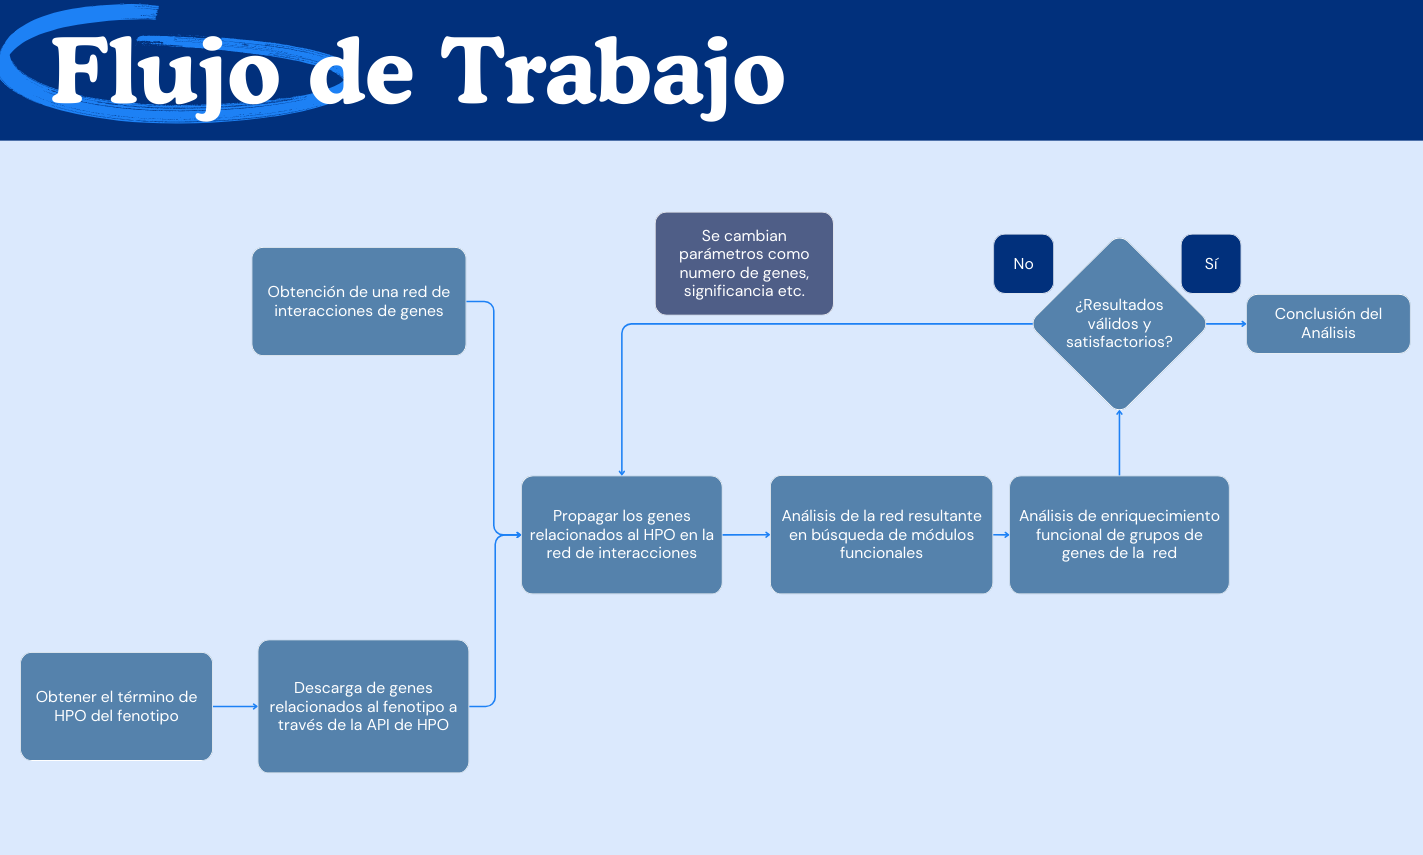
\includegraphics[width=.95\textwidth]{figures/workflow.png}
	\caption{Flujo de trabajo para obtener análisis de enriquecimiento mejorado del fenotipo signo de Hoffmann}
	\label{fig:workflow}
\end{figure}

\subsection{Obtención de genes relacionados con signo de Hoffmann}

Para obtener los genes relacionados con el signo de Hoffmann (HP:0031993), se utilizó la API de la Ontología de Fenotipos Humanos (HPO). El recurso consultado contiene nuestro termino HPO y el endpoint de genes (https://ontology.jax.org/api/
network/annotation/HP:0031993/download/gene). Mediante una solicitud HTTP, se extrajo y almacenó esta información en archivos con formato .tsv, facilitando así su posterior análisis. 


\subsection{Obtención de red de interacciones de genes}

Para el análisis de interacciones génicas, se utilizó una red de interacciones obtenida de la base de datos STRING. Las interacciones de proteínas humanas (\textit{Homo sapiens}, ID taxonómico: 9606) fueron descargadas de el endpoint de descargas de STRING (https://stringdb-downloads.org/download/prot ein.links.v12.0/9606.protein.links.v12.0.txt.gz). Solo se consideraron interacciones con una puntuación combinada (\textit{combined score}) mayor o igual a 400.

\subsection{Propagación de red}


Para identificar genes adicionales asociados al conjunto de genes iniciales relacionados con el Signo de Hoffmann, se aplicó el algoritmo de propagación de red DIAMOnD \cite{Ghiassian2015}. Se utilizó la red de interacciones génicas como base, y el algoritmo añadió nodos que optimizaban el índice hipergeométrico, una medida estadística que evalúa la probabilidad de que dos conjuntos tengan una superposición de elementos al menos tan grande como la observada, en comparación con lo que se esperaría por azar. En caso de empate, se empleó la suma ponderada de los pesos de las conexiones con los genes del grafo para desempatar, dando preferencia a los nodos con conexiones más relevantes y fuertemente conectados.


\subsection{Análisis de red}

Para el análisis de redes, se utilizó el algoritmo de Louvain \cite{Blondel2008} para detectar módulos funcionales en la red optimizando la partición de la red y maximizando su modularidad. Además, se implementaron métricas topológicas como la centralidad de grado, que mide el número de conexiones directas de cada nodo; la centralidad de intermediación, que identifica nodos clave en el flujo de información; y la centralidad de cercanía, que evalúa la proximidad de un nodo respecto al resto. Estas métricas, calculadas mediante la librería iGraph descrita en los materiales.

\subsection{Análisis de enriquecimiento funcional}

Una vez identificados los clusters, se realizó un análisis de enriquecimiento funcional con la herramienta Enrichr \cite{10.1093/nar/gkad393/1} que compara diferentes fuentes de datos para determinar qué funciones biológicas, rutas metabólicas o procesos celulares están sobrerrepresentados en los grupos de genes detectados.
